\subsection{Стохастическая чувствительность}

    Для аппроксимации вероятностного распределения случайных состояний вокур детерминированных аттракторов (равновеися или циклов) можно использовать сетод функции стохастический чувствительности. \comment{Смотри ВКР, там есть ссылка на книгу, стр 17}.

    \comment{Думаю формулы тут не нужны, мб оставить ссылку на статью Crises, noise, and tipping in the Hassell population model}

    На графике \ref{bifurcation_x_0_2_a_1_beta_chaos_fss} красными линиями нарисована ФСЧ. 

    % \begin{figure}
    %     \centering
    %     \includegraphics[width=\textwidth]{stochastic/bifurcation_x_0_2_a_1_beta_noise_fss.jpg}
        
    %     \captionsetup{justification=centering}
    %     \caption{График бифуркации с \(\beta\)-шумом.}
    %     \label{bifurcation_x_0_2_a_1_beta_chaos_fss}
    % \end{figure}

    \begin{figure}
        \centering
        \subfloat[Общий вид бифуркационной диаграммы с ФСЧ]{
            \includegraphics[width=0.7\textwidth]{stochastic/images/bifurcation_x_0_2_a_1_beta_noise_fss.jpg}
            \label{bifurcation_x_0_2_a_1_beta_chaos_fss}
        }

        \subfloat[ФСЧ для равновесия]{
            \includegraphics[width=0.5\textwidth]{stochastic/images/bifurcation_x_0_2_a_1_beta_noise_fss_segment_stable.jpg}
            \label{bifurcation_x_0_2_a_1_beta_chaos_fss_segment_stable}
        }  
        \subfloat[ФСЧ для 2-цикла]{
            \includegraphics[width=0.5\textwidth]{stochastic/images/bifurcation_x_0_2_a_1_beta_noise_fss_segment_2_cycle.jpg}
            \label{bifurcation_x_0_2_a_1_beta_chaos_fss_segment_2_cycle}
        }
            
        \subfloat[ФСЧ для хаоса]{
            \includegraphics[width=0.5\textwidth]{stochastic/images/bifurcation_x_0_2_a_1_beta_noise_fss_segment_chaos_up.jpg}
            \label{bifurcation_x_0_2_a_1_beta_chaos_fss_segment_chaos_up}
        }
        \subfloat[ФСЧ для хаоса]{
            \includegraphics[width=0.5\textwidth]{stochastic/images/bifurcation_x_0_2_a_1_beta_noise_fss_segment_chaos_down.jpg}
            \label{bifurcation_x_0_2_a_1_beta_chaos_fss_segment_chaos_down}
        }
            
        \caption{Бифуркационная диаграмма с ФСЧ}
    \end{figure}

    Рассмотрим участок от \(\beta \approx 0.45\) до \(\beta \approx 0.48\), он изображен на рисунке \ref{bifurcation_x_0_2_a_1_beta_chaos_fss_segment_stable}. Мы видим, что значения графика бифуркации почти всегда находятся в коридоре, границами которого являются значения ФСЧ. Этот коридор строится по правилу трех сигм. Такой подход гарантирует, что почти все значения будут находиться в этом интервале, что собственно мы и наблюдаем.

    % \begin{figure}
    %     \centering
    %     \includegraphics[width=\textwidth]{stochastic/bifurcation_x_0_2_a_1_beta_noise_fss_segment_stable.jpg}
        
    %     \captionsetup{justification=centering}
    %     \caption{}
    %     \label{bifurcation_x_0_2_a_1_beta_chaos_fss_segment_stable}
    % \end{figure}

    На участках с k-циклами и хаосом (рисунки \ref{bifurcation_x_0_2_a_1_beta_chaos_fss_segment_2_cycle}, \ref{bifurcation_x_0_2_a_1_beta_chaos_fss_segment_chaos_up} и \ref{bifurcation_x_0_2_a_1_beta_chaos_fss_segment_chaos_down]}) будет наблюдаться аналогичная ситуация: значения лежат в коридоре, ограниченном значениями ФСЧ.

    % \begin{figure}
    %     \centering
    %     \includegraphics[width=\textwidth]{stochastic/bifurcation_x_0_2_a_1_beta_noise_fss_segment_2_cycle.jpg}
        
    %     \captionsetup{justification=centering}
    %     \caption{}
    %     \label{bifurcation_x_0_2_a_1_beta_chaos_fss_segment_2_cycle}
    % \end{figure}

    % \begin{figure}
    %     \centering
    %     \includegraphics[width=\textwidth]{stochastic/bifurcation_x_0_2_a_1_beta_noise_fss_segment_chaos_up.jpg}
        
    %     \captionsetup{justification=centering}
    %     \caption{}
    %     \label{bifurcation_x_0_2_a_1_beta_chaos_fss_segment_chaos_up}
    % \end{figure}

    % \begin{figure}
    %     \centering
    %     \includegraphics[width=\textwidth]{stochastic/bifurcation_x_0_2_a_1_beta_noise_fss_segment_chaos_down.jpg}
        
    %     \captionsetup{justification=centering}
    %     \caption{}
    %     \label{bifurcation_x_0_2_a_1_beta_chaos_fss_segment_chaos_down}
    % \end{figure}
